\chapter{Discussion}

\begin{figure}[h!]
    \centering
    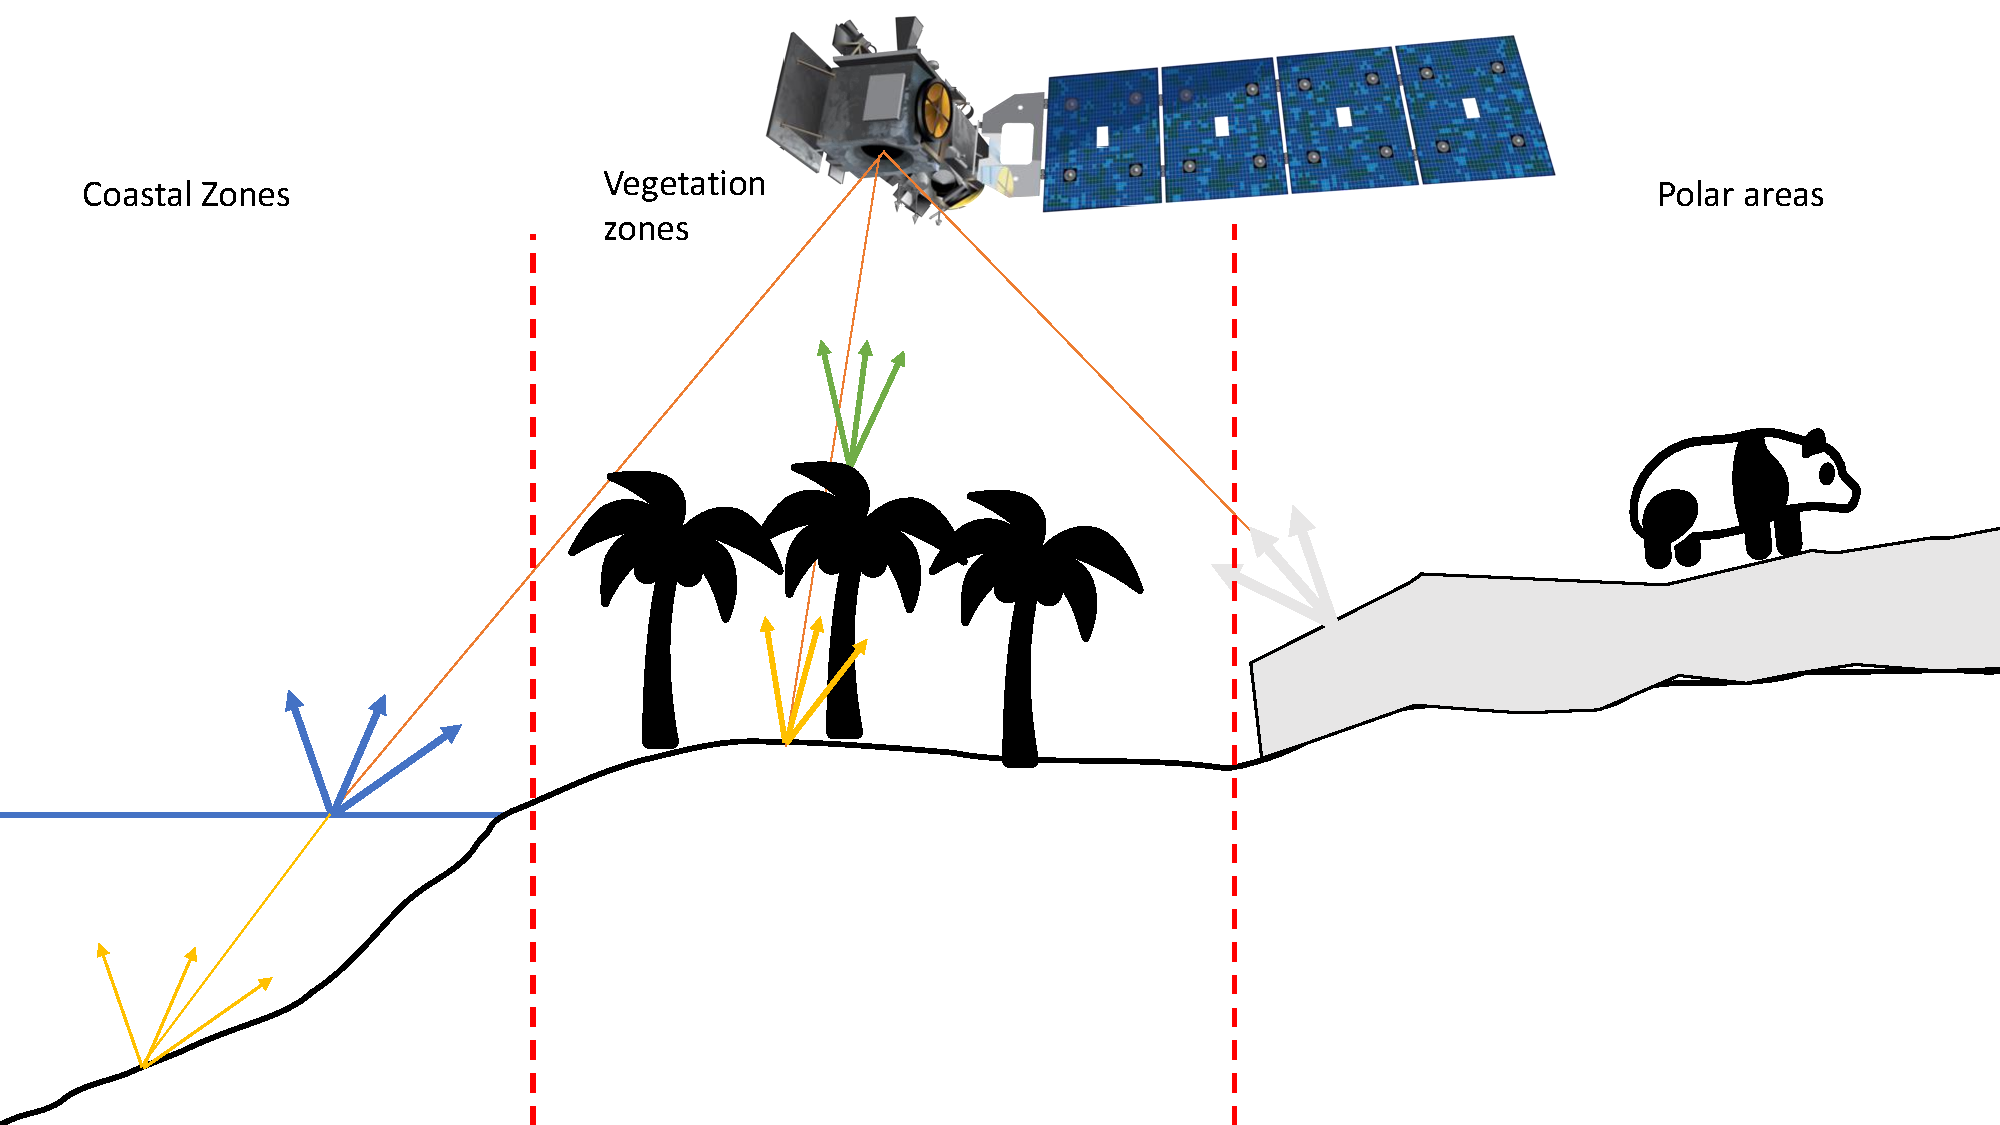
\includegraphics[width=0.75\textwidth]{figures/summary.pdf}
    \caption{Overview}\pdfcomment{obviously this is a pretty rough draft ;) }
    \label{fig:icesat-summary-image}
\end{figure}


\section{A-priori identification of transects with useful bathymetric signal}
\pdfcomment{I think i need to make it clearer in my abstract that this is a goal} One of the goals of the project is to find a way to predict nearshore zones which are most likely to have ICESat-2 bathymetry available before downloading the photon-level data and running the KDE signal finding algorithm. A-priori identification of promising sites is useful to minimize the computing resources required when scaling up the approach to a global level.

In looking at the transect data as a whole, there was not one clear variable which predicts either the availability of bathymetric data, or the quality  (measured by RMSE) of data an individual lidar transect. It is well-established that lidar and optical bathymetry are highly sensitive to turbidity levels, since they require light to be able to reach the seafloor. It was hypothesized that the Secchi depth, as estimated by optical satellite methods, would be a reliable indicator of bathymetric quality and quantity for a given transect. However, no clear relationship was found between the Secchi depth and the quality and quantity of bathymetric signal photons. In fact, the Florida Keys test site has the lowest median Secchi depth (8.3m) of any of the test sites investigated, while also providing among the highest quality data (0.87m RMSE), and the largest percent of transects containing good data of any test sites. 

The most likely explanation for this seeming paradox is that the characteristics that make a site ideal for ICESat-2 bathymetry --- a wide, shallow shelf with clear water --- could affect the accuracy of optical ocean color measurements. The area of interest selected in the Florida Keys site has large areas with a depth of less than 10m, and exceptionally clear water. The Secchi depth determination is based on passive optical remote sensing response of the site. It is possible that because in this site there is a very significant amount of sunlight reflecting from the seabed, the Secchi depth algorithms used in the GlobColour product have limited accuracy. This is further supported by the fact that the Secchi depth uncertainty metric (median 56\% uncertainty) is much higher for the Florida Keys site than any other site. Table \ref{tab:ocean_color_summary_by_site} shows the median secch depth and light diffusion coefficient for each subsite, as well as the RMSE and MAE error between the ICESat-2 point data and the validation data.


\begin{table}
    \centering
    \caption{Secchi Depth and RMSE for each site}
    \label{tab:ocean_color_summary_by_site}
    \begin{tabular}{lrrrrrr}
        \toprule
        {}
        Site Name           & $Zsd_{50}$[m] & $\sigma_{Zsd_{50}}$ & RMS Error [m] & MAE [m] & ME [m] \\
        \midrule
        St. Thomas/St. John & 23.52         & 23.92               & 1.08          & 0.56    & -0.17  \\
        Florida Keys        & 8.29          & 56.01               & 0.79          & 0.31    & 0.24   \\
        Oahu 1              & 29.70         & 29.52               & 1.16          & 0.77    & 0.54   \\
        Oahu 2              & 31.59         & 28.97               & 10.60         & 1.45    & 1.41   \\
        Oahu 3              & 28.43         & 50.92               & 1.24          & 0.46    & 0.30   \\
        Oahu 4              & 28.43         & 27.14               & 0.61          & 0.39    & 0.26   \\
        Oahu 5              & 29.84         & 25.48               & 0.73          & 0.50    & 0.27   \\
        Oahu 6              & 28.93         & 31.82               & 2.42          & 1.76    & -1.43  \\
        Oahu 7              & 32.76         & 25.54               & 1.11          & 0.72    & -0.02  \\
        Oahu 8              & 33.26         & 23.75               & 0.67          & 0.52    & 0.35   \\
        St. Croix           & 26.89         & 41.20               & 0.54          & 0.30    & -0.11  \\
        \bottomrule
    \end{tabular}
\end{table}


\section{Bathymetry extraction from ICESat-2 lidar}

Compared to other signal finding methods proposed the literature, the implementation used here results in a similar order of RMSE for most of the test sites. The KDE signal finding method proposed was able to identify bathymetric photons with an RMSE of between 0.54m and 9.53m RMSE. This is a very wide range of reliability, and would require further refinement before scaling the method to more sites. The site with the largest error was in an area with steep cliffs on the south end of Oahu, Hawai'i. The source of the error was a failure in the photon filtering approach \pdfcomment{explain with figure}. The error was caused by some points with a true elevation of 118m being labeled as subsurface photons. Because they are in a land area, they should have been removed by the GEBCO filtering step. However, because of the limited horizontal accuracy of GEBCO data they were not removed from the photon cloud during subsurface photon filtering.

The best way to mitigate this would be to find a better land mask dataset. This is likely possible for sites in the global north that have good data availability, but higher resolution land masks might not be available in the entire world. It should be noted that the ATL03 dataset does include a surface mask flag as one of the variables. However, it is not suitable for this purpose because there is an intentional overlap between the boundaries of these different masks. Therefore, a photon return in a coastal zone can be classified as being both in the ocean, land, and inland water zones. This is done because it is assumed there is a high uncertainty in the exact boundaries between surface types. 

One of the major challenges to the proposed KDE signal finding method is that it is very sensitive to the input parameters, especially the threshold local density to consider a point to be valid signal. The assumption used here was set empirically, and it was the greater of either a.) the median KDE of the transect, or b.) 0.1. By making this criterion stricter (increasing the minimum to 0.15) the RMSE error at each site is reduced significantly. However, this presents a tradeoff. While a few large magnitude errors are filtered out by this method, there are many times more high-quality points that are also excluded. By excluding these points, it often reduces the overall spatial distribution of the resulting point data (the KDE is correlated for a given transect, so by increasing the threshold, often entire transects worth of points are removed). Therefore, increasing this threshold is quite a blunt instrument that removes significant amounts of high quality data. It was found that using a lower density threshold, and therefore allowing some large errors to remain in the point data, the overall quality of the kriging interpolation and the resulting Kalman-updated was improved. 

One potential avenue for improving the discretion of the algorithm would be considering the local horizontal density of photon returns. A rolling window based on distance rather than a set number of adjacent photons could potentially improve the quality of the KDE magnitude estimation. Another approach might be to normalize the KDE value based on the transect length, and see if that improves the ability to throw out low-quality data while retaining high-quality data.

It is possible that the results could be further improved by building a larger dataset of validation sites, and trying to find globally optimum parameters that provide a good balance of excluding low accuracy points and maintaining as much quality data as possible.

\section{2D interpolation via universal kriging}

The universal kriging approach proved effective to transform the point estimates into a gridded estimate of seabed elevation and uncertainty. 

The largest practical limitation to the Bayesian updating method is the requirement to interpolate the data. Kriging interpolaters are ideal because they are robust to outliers and provide an uncertainty estimate as well as a depth estimate. The downside of the kriging interpolator is both the computational complexity and the requirement that points are not too close together. If points are too close to one another, the kriging matrix is not soluble, and the algorithm has a complexity of $\mathcal{O}(n^3)$ where $n$ is the number of points. This means that there is a relatively strict practical limitation to the number of points that can be used as input to the interpolator. The upper limit with a laptop with 32GB RAM was found to be approximately 2000 points without exceeding the available memory. One way to deal with this is to use a tiling strategy, and repeat the process using tiles which contain 2000 bathymetric points or less. This would need to be done adaptively since the bathymetric points are not evenly distributed. Using a larger number of smaller sub-sites would take longer to process, but it would at least be feasible using a consumer-grade computer.

One disadvantage of ICESat-2 data is the uneven spatial distribution of the resulting bathymetric points. Due to the orbit of ICESat-2, the ATL03 data is available along transects oriented $\pm \ang{6}$ relative to north (see Figure \ref{fig:distribution-of-bathy-points-in-space}). Because of this pattern, even if there was perfect bathymetry data along every single ICESat-2 transect within the study area, the spatial distribution of the points would be anisotropic. Given that there are gaps in these transects where the bathymetric signal is weaker, the spatial distribution of the data can vary significantly by site. These gaps along transects can be seen in Figure \ref{fig:distribution-of-bathy-points-in-space}. The gaps of weaker signal can be caused by areas that are too deep or too turbid for the laser to reach the seabed, or due to instrument/atmospheric issues (\ref{sec:discussion-photon-issues}). 


\begin{figure}
    \pdfcomment{redo in cartopy/add scale bar/other map stuff}
    \centering
    \includegraphics[width=0.75\textwidth]{figures/temp_spatial_dist.png}
    \caption{Spatial distribution of bathymetry points in St. Croix north end, and the true bathymetry. The red lines show transects. The north end of the transects in this figure are cut off by the request polygon. The blue dots show the locations of bathymetric signal as identified by the KDE signal finding algorithm.}
    \label{fig:distribution-of-bathy-points-in-space}
\end{figure}

However, handling this uneven spatial distribution is one of the advantages of using a geostatisical approach. Areas that are distant from any input points have a higher uncertainty in the output grid, and therefore there is little or no change from the prior estimate, since the Kalman update step accounts for the estimate uncertainty. Therefore, in locations that are further away from valid data, there is little or no change from the prior estimate. A limitation of this is that any accuracy gains are might not be evenly distributed across the site. 

\section{Kalman updating and improvement over GEBCO}

It was found that in most sites, the Bayesian combination of bilinearly resampled GEBCO data and the interpolated ICESat-2 data increased the accuracy compared to the validation data than either product on their own. The average decrease in RMSE was on the order of 30\% \pdfcomment{going to crunch the numbers again but this is close}

The optimal decrease in RMSE error was found by assuming a GEBCO uncertainty of $\sigma=1.5m$ standard deviation. This produced the best results for the test sites under consideration, however the actual GEBCO uncertainty depends on myriad factors including the original data source, survey method, and how old it is. One improvement that could be further explored is how the uncertainty of GEBCO varies with the Type IDentifier (TID) grid. The TID is a GEBCO data product that indicates the original source of the data. It is likely that the original data source affects the error between the GEBCO grid and the validation data.

One limitation is that the temporal resolution of the ICESat-2 data is not sufficient to take full advantage of the Kalman filtering approach, which normally includes updates both in space and time. The satellite repeat time for a given reference ground track is 91 days, and the data is available starting in 2018. Due to off-pointing over most land areas, there is often greater than 91 days between passes of the \emph{exact same} track. Since coasts are among the most dynamic morphological environments, there might be substantial changes between repeat passes. The proposed method assumes that the all the bathymetry data is contemporaneous. This is an inherent limitation to the method, since it cannot account for morphological changes that might occur during the 4-year time window in which the data was collected. However, the ICESat-2 data is very likely more recent than the input data to the GEBCO gridding process, which in some places can come from digitized nautical maps that can be hundreds of years old. Therefore, all data was assumed to be contemporaneous, and the time update step of the Kalman Filter was not used.


One potential downside of the Bayesian update approach is that it could create artifacts in the resulting output data, even if the RMS error is decreased relative to GEBCO. If there is an area with a high density of incorrect point measurements, the resulting uncertainty data might have a high confidence in that local area, leading to a significant update to the prior estimate which does not reflect a physical seabed  feature. This effect could create artificial shoals or shallow areas. \pdfcomment{this probably needs a graphic to help explain} Because the RMSE error is decreasing relative to the validation data, we know that the \emph{net} effect of the Bayesian update is an improvement. However, the addition of phantom shoals could make the data nearly useless for numerical modeling studies, since introducing an artificial high point offshore could change the wave transformation significantly. However, the decreased average error of the resulting product could still could have utility for estimating dredging quantities, which are less sensitive to an individual high point. 